\documentclass[11pt]{article}
\usepackage[margin=0.8in]{geometry}
\usepackage{amsmath,amssymb,booktabs,array,longtable}
\usepackage{graphicx}
\usepackage{hyperref}
\usepackage{enumitem}
\setlist{nosep}

\begin{document}

\begin{center}
{\Large\textbf{Shiv Nadar University Chennai}}\\
\textbf{CS3807 -- Deep Learning Laboratory}\\
\textbf{Experiment 3}\\
{\large\textbf{Implementation of Convolutional Neural Networks (CNNs) for Image Classification}}
\end{center}

\renewcommand{\arraystretch}{1.25}

\begin{tabular}{|p{3.8cm}|p{8cm}|p{2cm}|}
\hline
Degree \& Branch & B.Tech Artificial Intelligence \& Data Science & Semester V\\ \hline
Subject Code \& Name & CS3807 -- Deep Learning Laboratory & AY: 2026--27\\ \hline
\end{tabular}

\vspace{4mm}
Name : Ashwin S\\
Reg no : 24011101007\\
Class : AI DS - A (batch 1)\\

\vspace{6mm}
\section*{1. Objective}
To understand the working principle of Convolutional Neural Networks by implementing convolution, pooling, feature map visualization, and image classification using TensorFlow/Keras.

\vspace{6mm}
\section*{2. Theory}
A Convolutional Neural Network consists of

\begin{itemize}
\item Convolution Layer
\item Activation Layer
\item Pooling Layer
\item Fully Connected Layer
\end{itemize}

The convolution operation is
\[
Y(i,j)=\sum_m\sum_n X(i+m,j+n)K(m,n)
\]
where

\begin{itemize}
\item $X$ : Input Image
\item $K$ : Kernel (Filter)
\item $Y$ : Feature Map
\end{itemize}

The output feature map size is
\[
\frac{N-F+2P}{S}+1
\]
where $N$ is Input Size, $F$ is Filter Size, $P$ is Padding, $S$ is Stride.

\vspace{4mm}
\subsection*{Common Convolution Kernels}

A kernel (or filter) is a small matrix that slides over an input image to extract important visual features such as edges, textures, corners, and smooth regions. During convolution, the kernel is multiplied element-wise with the corresponding image pixels, and the results are summed to produce a single value in the output feature map. Different kernels highlight different image characteristics.

\vspace{3mm}
\paragraph{1. Identity Kernel}
The identity kernel preserves the original image without modifying its pixel values.
\[
\begin{bmatrix} 0 & 0 & 0 \\ 0 & 1 & 0 \\ 0 & 0 & 0 \end{bmatrix}
\]
Purpose:
\begin{itemize}
\item Preserves the original image.
\item Used for understanding the convolution operation.
\end{itemize}

\vspace{3mm}
\paragraph{2. Sobel-X Kernel (Vertical Edge Detection)}
The Sobel-X kernel detects vertical edges by measuring intensity changes along the horizontal direction.
\[
\begin{bmatrix} -1 & 0 & 1 \\ -2 & 0 & 2 \\ -1 & 0 & 1 \end{bmatrix}
\]
Applications:
\begin{itemize}
\item Object detection
\item Lane detection
\item Face recognition
\end{itemize}

\vspace{3mm}
\paragraph{3. Sobel-Y Kernel (Horizontal Edge Detection)}
The Sobel-Y kernel detects horizontal edges by measuring intensity changes along the vertical direction.
\[
\begin{bmatrix} -1 & -2 & -1 \\ 0 & 0 & 0 \\ 1 & 2 & 1 \end{bmatrix}
\]
Applications:
\begin{itemize}
\item Text detection
\item Boundary extraction
\item Medical image analysis
\end{itemize}

\vspace{3mm}
\paragraph{4. Laplacian Kernel}
The Laplacian kernel detects edges in all directions using the second-order derivative of image intensity.
\[
\begin{bmatrix} 0 & -1 & 0 \\ -1 & 4 & -1 \\ 0 & -1 & 0 \end{bmatrix}
\]
Applications:
\begin{itemize}
\item Edge enhancement
\item Satellite image analysis
\item Medical imaging
\end{itemize}

\vspace{3mm}
\paragraph{5. Sharpening Kernel}
This kernel enhances fine details by emphasizing high-frequency components.
\[
\begin{bmatrix} 0 & -1 & 0 \\ -1 & 5 & -1 \\ 0 & -1 & 0 \end{bmatrix}
\]
Applications:
\begin{itemize}
\item Image enhancement
\item Optical Character Recognition (OCR)
\item Face recognition
\end{itemize}

\vspace{3mm}
\paragraph{6. Box Blur Kernel}
The Box Blur kernel smooths an image by replacing each pixel with the average of its neighboring pixels.
\[
\frac{1}{9}\begin{bmatrix} 1 & 1 & 1 \\ 1 & 1 & 1 \\ 1 & 1 & 1 \end{bmatrix}
\]
Applications:
\begin{itemize}
\item Noise removal
\item Image smoothing
\item Image preprocessing
\end{itemize}

\vspace{3mm}
\paragraph{7. Gaussian Blur Kernel}
Gaussian blur smooths the image while preserving the overall structure better than a simple average filter.
\[
\frac{1}{16}\begin{bmatrix} 1 & 2 & 1 \\ 2 & 4 & 2 \\ 1 & 2 & 1 \end{bmatrix}
\]
Applications:
\begin{itemize}
\item Noise reduction
\item Computer vision preprocessing
\item Feature extraction
\end{itemize}

\vspace{3mm}
\paragraph{8. Emboss Kernel}
The Emboss kernel creates a three-dimensional appearance by emphasizing directional changes in intensity.
\[
\begin{bmatrix} -2 & -1 & 0 \\ -1 & 1 & 1 \\ 0 & 1 & 2 \end{bmatrix}
\]
Applications:
\begin{itemize}
\item Texture analysis
\item Artistic image effects
\end{itemize}

\vspace{3mm}
\paragraph{9. Outline Detection Kernel}
This kernel highlights object boundaries by emphasizing regions with rapid intensity changes.
\[
\begin{bmatrix} -1 & -1 & -1 \\ -1 & 8 & -1 \\ -1 & -1 & -1 \end{bmatrix}
\]
Applications:
\begin{itemize}
\item Image segmentation
\item Boundary detection
\item Shape extraction
\end{itemize}

\vspace{3mm}
\paragraph{10. Motion Blur Kernel}
This kernel simulates motion blur along the diagonal direction.
\[
\frac{1}{5}
\begin{bmatrix}
1 & 0 & 0 & 0 & 0 \\
0 & 1 & 0 & 0 & 0 \\
0 & 0 & 1 & 0 & 0 \\
0 & 0 & 0 & 1 & 0 \\
0 & 0 & 0 & 0 & 1
\end{bmatrix}
\]
Applications:
\begin{itemize}
\item Motion simulation
\item Image restoration
\item Video processing
\end{itemize}

\vspace{4mm}
\subsection*{Summary of Common Kernels}

\begin{center}
\begin{tabular}{|p{2.6cm}|p{1.3cm}|p{5.3cm}|p{5cm}|}
\hline
\textbf{Kernel} & \textbf{Size} & \textbf{Purpose} & \textbf{Applications}\\
\hline
Identity & $3\times3$ & Preserve original image & Baseline comparison\\
\hline
Sobel-X & $3\times3$ & Detect vertical edges & Object detection\\
\hline
Sobel-Y & $3\times3$ & Detect horizontal edges & Boundary detection\\
\hline
Laplacian & $3\times3$ & Detect edges in all directions & Medical imaging\\
\hline
Sharpen & $3\times3$ & Enhance details & Image enhancement\\
\hline
Box Blur & $3\times3$ & Smooth image & Noise removal\\
\hline
Gaussian Blur & $3\times3$ & Reduce noise & Computer vision\\
\hline
Emboss & $3\times3$ & 3D effect & Artistic filtering\\
\hline
Outline & $3\times3$ & Boundary extraction & Segmentation\\
\hline
Motion Blur & $5\times5$ & Simulate motion & Video processing\\
\hline
\end{tabular}
\end{center}

\vspace{4mm}
\subsection*{Numerical Example 1: Convolution}

Consider the following input image.
\[
X=\begin{bmatrix}1&2&3\\4&5&6\\7&8&9\end{bmatrix}
\]

Kernel
\[
K=\begin{bmatrix}1&0\\0&1\end{bmatrix}
\]

Output

First position\\
$1(1)+2(0)+4(0)+5(1)=6$

Second position\\
$2(1)+3(0)+5(0)+6(1)=8$

Third position\\
$4(1)+5(0)+7(0)+8(1)=12$

Fourth position\\
$5(1)+6(0)+8(0)+9(1)=14$

Feature Map
\[
\begin{bmatrix}6&8\\12&14\end{bmatrix}
\]

\vspace{4mm}
\subsection*{Numerical Example 2: Max Pooling}

Feature map
\[
\begin{bmatrix}1&5&2&3\\7&8&1&0\\4&6&9&5\\2&3&1&8\end{bmatrix}
\]

Using a $2\times2$ max pooling filter,

Window 1
\[
\begin{bmatrix}1&5\\7&8\end{bmatrix}\rightarrow8
\]

Window 2
\[
\begin{bmatrix}2&3\\1&0\end{bmatrix}\rightarrow3
\]

Window 3
\[
\begin{bmatrix}4&6\\2&3\end{bmatrix}\rightarrow6
\]

Window 4
\[
\begin{bmatrix}9&5\\1&8\end{bmatrix}\rightarrow9
\]

Output
\[
\begin{bmatrix}8&3\\6&9\end{bmatrix}
\]

\vspace{4mm}
\subsection*{Numerical Example 3: Parameter Calculation}

Suppose

Input Image\\
$32\times32\times3$

Convolution Layer
\begin{itemize}
\item Filters = 16
\item Kernel = $3\times3$
\end{itemize}

Parameters
\[
(3\times3\times3+1)\times16=(27+1)\times16=448
\]

Therefore, total trainable parameters $=448$.

\vspace{6mm}
\section*{3. Dataset}
Dataset: CIFAR-10

\begin{itemize}
\item Training Images: 50,000
\item Testing Images: 10,000
\item Classes: 10
\item Image Size: $32\times32\times3$
\end{itemize}

Dataset source: \url{https://www.kaggle.com/datasets/pankrzysiu/cifar10-python}

\vspace{6mm}
\section*{4. Experimental Procedure}

\textbf{Task 1}

Load CIFAR-10.
\begin{itemize}
\item Display ten sample images.
\item Print dataset dimensions.
\item Plot class distribution.
\end{itemize}

\vspace{4mm}
\textbf{Task 2}

Implement a convolution layer.
\begin{itemize}
\item Compare Kernel $=3\times3$
\item Compare Kernel $=5\times5$
\item Compare Kernel $=7\times7$
\item Record feature map sizes.
\end{itemize}

\vspace{4mm}
\textbf{Task 3}

Study hyperparameters.
\begin{itemize}
\item Compare Stride $=1$
\item Compare Stride $=2$
\item Compare Padding $=$ Same
\item Compare Padding $=$ Valid
\item Compute output dimensions.
\end{itemize}

\vspace{4mm}
\textbf{Task 4}

Visualize feature maps after the first convolution layer.
\begin{itemize}
\item Display at least eight feature maps.
\end{itemize}

\vspace{4mm}
\textbf{Task 5}

Compare Max Pooling and Average Pooling.
\begin{itemize}
\item Compare output size.
\item Compare accuracy.
\end{itemize}

\vspace{4mm}
\textbf{Task 6}

Construct the following CNN:

\begin{center}
Input $\rightarrow$ Conv $\rightarrow$ ReLU $\rightarrow$ MaxPool $\rightarrow$ Conv $\rightarrow$ ReLU $\rightarrow$ MaxPool $\rightarrow$ Flatten $\rightarrow$ Dense $\rightarrow$ Softmax
\end{center}

Train for
\begin{itemize}
\item Optimizer: Adam
\item Epochs: 20
\item Batch Size: 32
\end{itemize}

\vspace{4mm}
\textbf{Task 7}

Evaluate
\begin{itemize}
\item Accuracy
\item Precision
\item Recall
\item F1-score
\item Confusion Matrix
\item Classification Report
\end{itemize}

\vspace{6mm}
\section*{5. Source Code}

The complete implementation, including data preprocessing, convolution and pooling experiments, model construction, training, evaluation, and the additional exercises, is available in the following repository:\\


\url{https://github.com/Ashwin271206/dl-lab/tree/main/Lab%203}\\

The repository contains a single Google Colab notebook covering all tasks experimented in this report, along with the generated figures.

\vspace{6mm}
\section*{6. Results}

\begin{center}
\renewcommand{\arraystretch}{1.5}
\begin{tabular}{|p{7cm}|p{4cm}|}
\hline
\textbf{Metric} & \textbf{Value}\\
\hline
Training Accuracy & 0.7310\\
\hline
Testing Accuracy & 0.7194\\
\hline
Precision & 0.7353\\
\hline
Recall & 0.7194\\
\hline
F1-score & 0.7179\\
\hline
Number of Trainable Parameters & 545,546\\
\hline
\end{tabular}
\end{center}

\vspace{6mm}
\section*{7. Plots \& Inferences}

\textbf{Sample Images}

\begin{center}
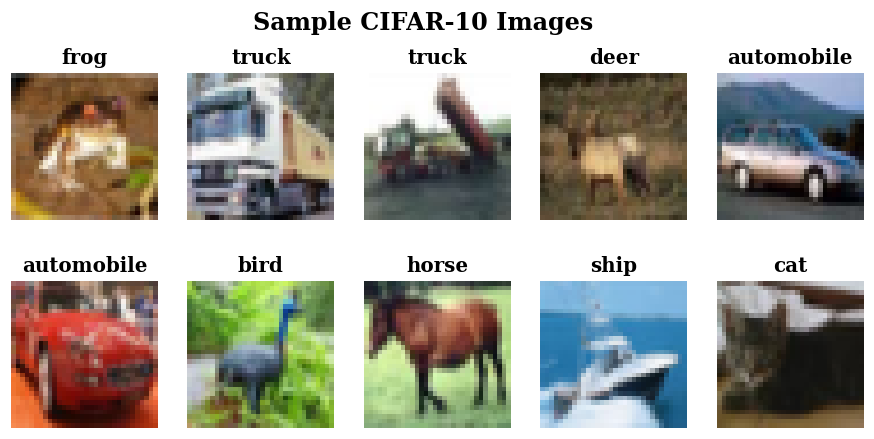
\includegraphics[width=0.8\textwidth]{figures/01_sample_images.png}
\end{center}

The sample image grid was generated successfully, indicating that the dataset is fully loaded and labelled correctly. These $32\times32$ RGB images correspond to the ten expected CIFAR-10 categories such as airplane, automobile, bird, and dog, confirming that the dataset is read in the expected format.

\vspace{4mm}
\textbf{Class Distribution}

\begin{center}
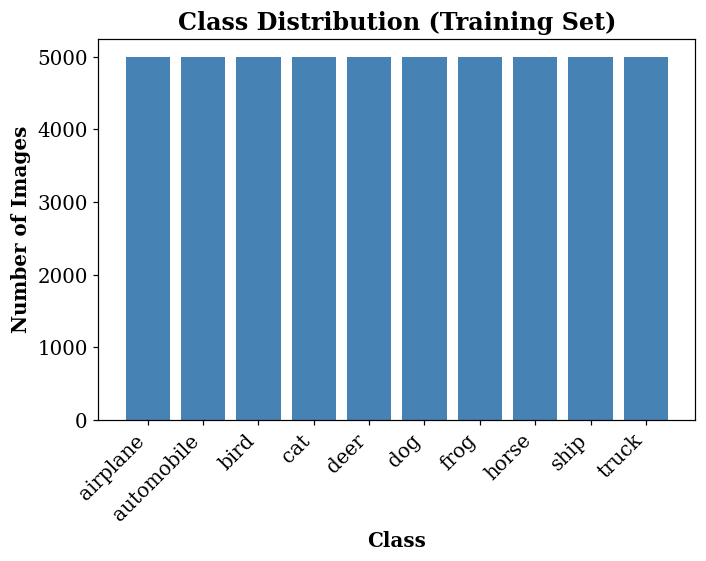
\includegraphics[width=0.8\textwidth]{figures/02_class_distribution.png}
\end{center}

All ten classes have an equal number of training samples, confirming that CIFAR-10 is a balanced dataset. This equal distribution means that evaluation metrics are fair across all classes, and no class-balancing technique is required.

\vspace{4mm}
\textbf{Kernel Size Comparison}

\begin{center}
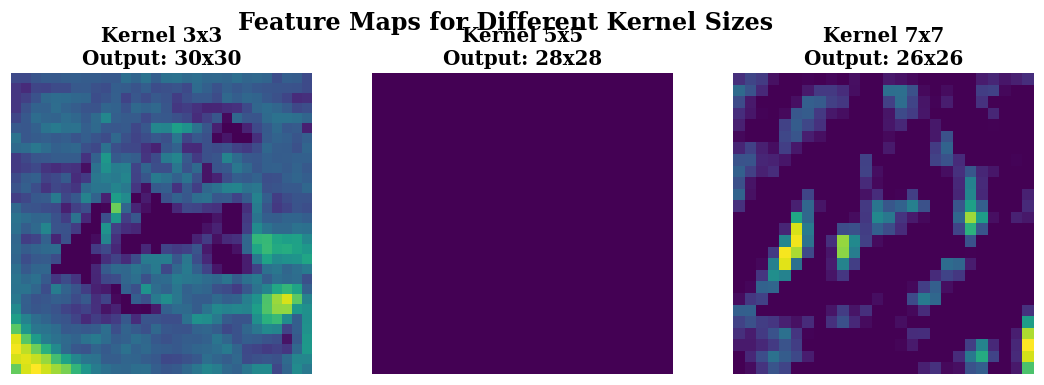
\includegraphics[width=0.8\textwidth]{figures/03_kernel_size_comparison.png}
\end{center}

As kernel size increases from $3\times3$ to $7\times7$, the resulting feature map becomes smaller and captures more global spatial patterns. Smaller kernels preserve finer spatial detail and are computationally cheaper, while larger kernels detects larger patterns over space.

\vspace{4mm}
\textbf{Stride and Padding Comparison}

\begin{center}
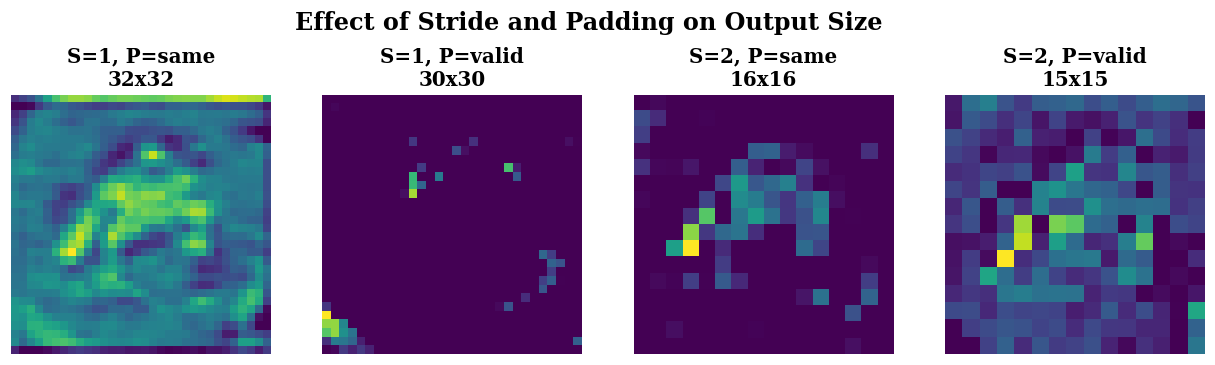
\includegraphics[width=0.8\textwidth]{figures/04_stride_padding_comparison.png}
\end{center}

Increasing stride from 1 to 2 approximately halves the output spatial dimension, directly reducing computation in subsequent layers. \texttt{same} padding preserves the input spatial size at stride 1, while \texttt{valid} padding shrinks it, matching the theoretical output-size formula.

\vspace{100mm}
\textbf{Feature Maps after First Convolution}

\begin{center}
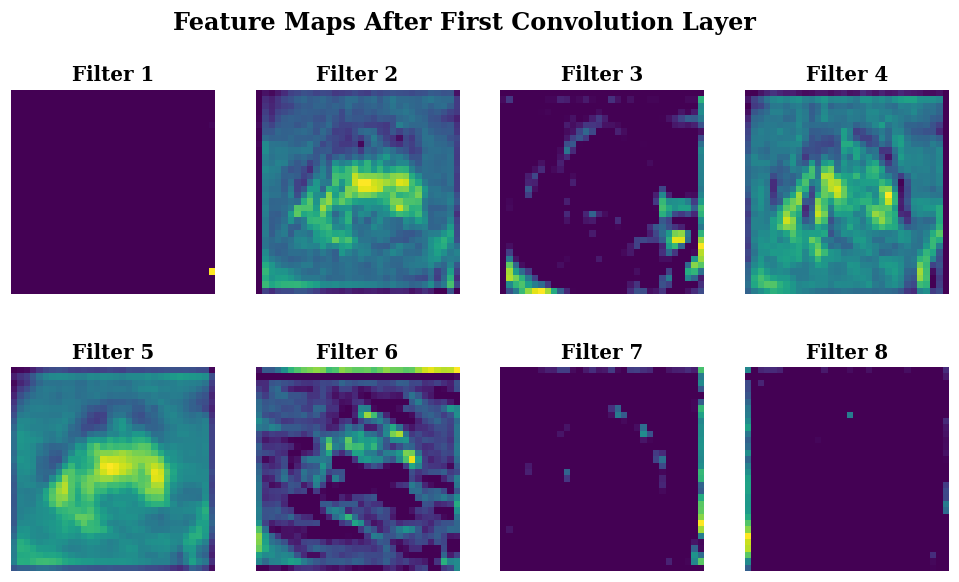
\includegraphics[width=0.8\textwidth]{figures/05_feature_maps_conv1.png}
\end{center}

Each feature map highlights a different learned pattern in the input image, such as edges, colour-contrast regions, or texture blobs. This shows that a single convolution layer extracts diverse, complementary representations of the same input image.

\vspace{4mm}
\textbf{Max Pooling vs Average Pooling -- Output Comparison}

\begin{center}
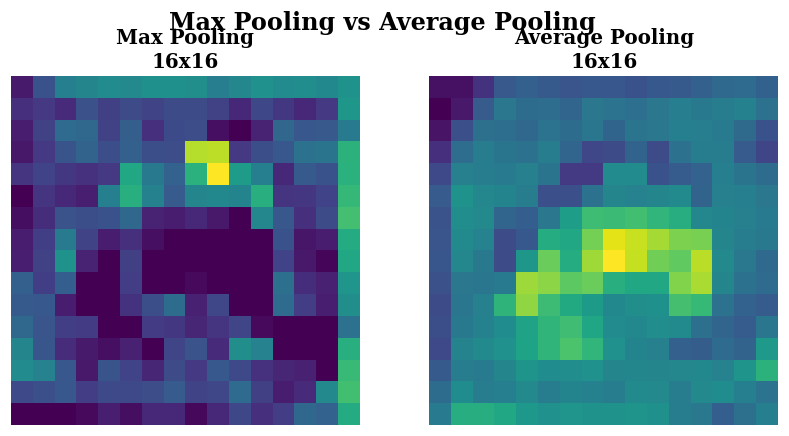
\includegraphics[width=0.8\textwidth]{figures/06_maxpool_vs_avgpool.png}
\end{center}

Max Pooling retains the largest activation in each window, and it captures the sharp features like edges, corners, etc. Average Pooling produces a smoothened output by averaging all values in the window, and gives stable, generalized outputs.

\vspace{20mm}
\textbf{Training Accuracy vs Epoch}

\begin{center}
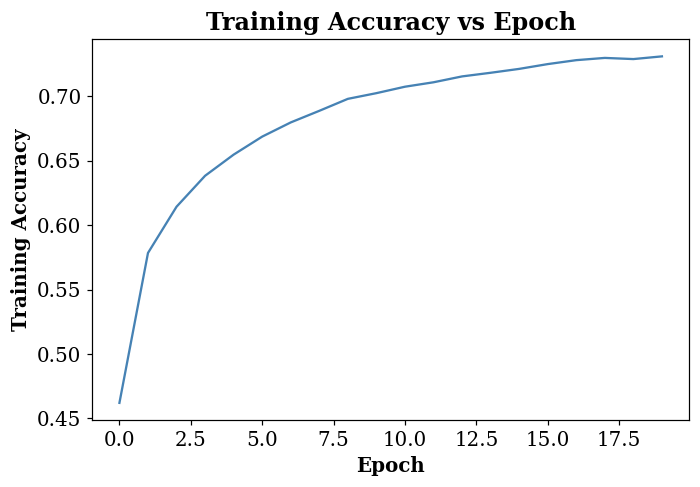
\includegraphics[width=0.8\textwidth]{figures/07_training_accuracy.png}
\end{center}

Training accuracy increases steadily across 20 epochs and the model learns contiunously. It surges in the beginning and slows down during later epochs, and starts to stabilize around epoch 18-20, approaching convergence.

\vspace{4mm}
\textbf{Validation Accuracy vs Epoch}

\begin{center}
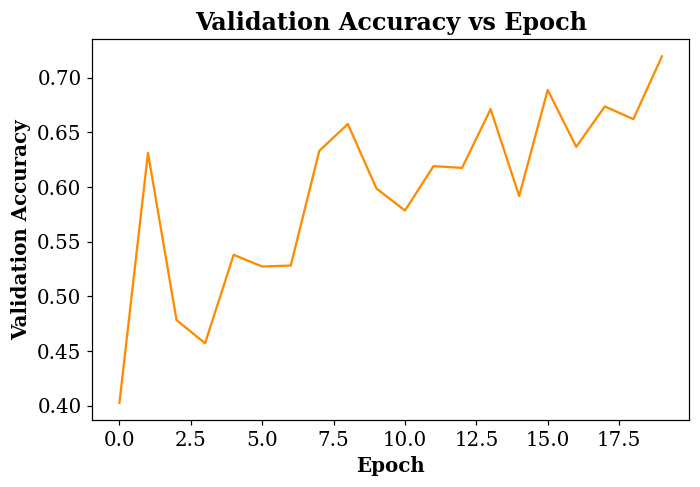
\includegraphics[width=0.8\textwidth]{figures/08_validation_accuracy.png}
\end{center}

Validation accuracy follows the path of training accuracy, but contains more fluctuations, reflecting the model's generalization performance on unseen data. Final accuracies are similar during training and validation, but for further epochs, if validation accuracy drops, it indicates overfitting. 

\vspace{4mm}
\textbf{Training Loss vs Epoch}

\begin{center}
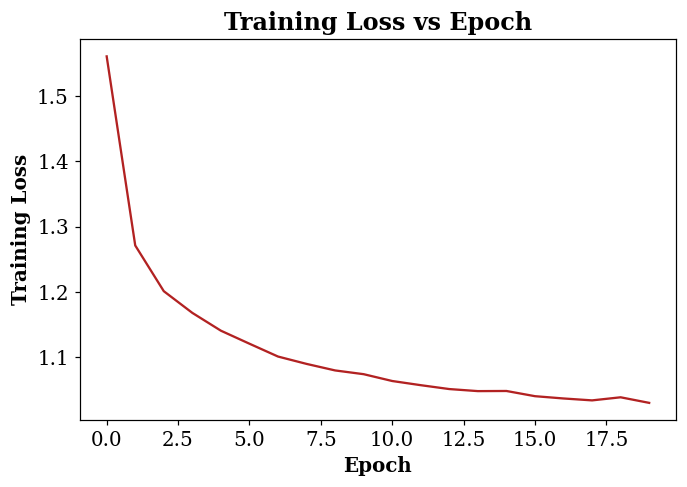
\includegraphics[width=0.8\textwidth]{figures/09_training_loss.png}
\end{center}

Training loss decreases consistently as epochs increase. This indicates the efficiency of Adam optimizer, as it proves to minimize the cross-entropy loss between true and predicted labels.

\vspace{4mm}
\textbf{Validation Loss vs Epoch}

\begin{center}
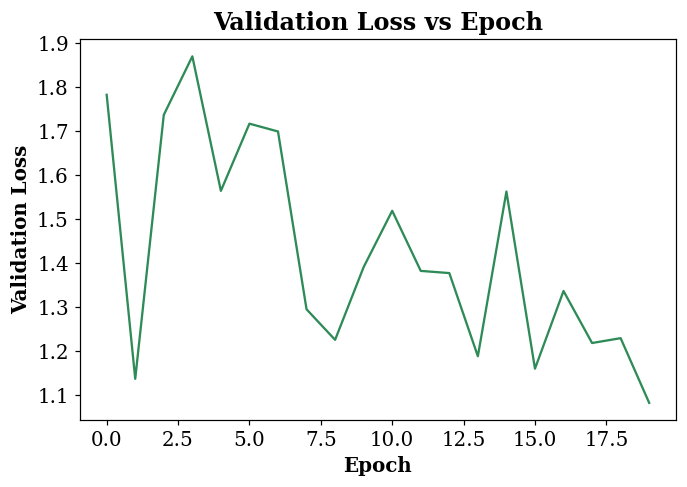
\includegraphics[width=0.8\textwidth]{figures/10_validation_loss.png}
\end{center}

Validation loss has decreased from epoch 1 to 20, but with heavy fluctuations. It does not stabilize anywhere, and it can learn further. A rise over further epochs would indicate overfitting.

\vspace{4mm}
\textbf{Confusion Matrix}

\begin{center}
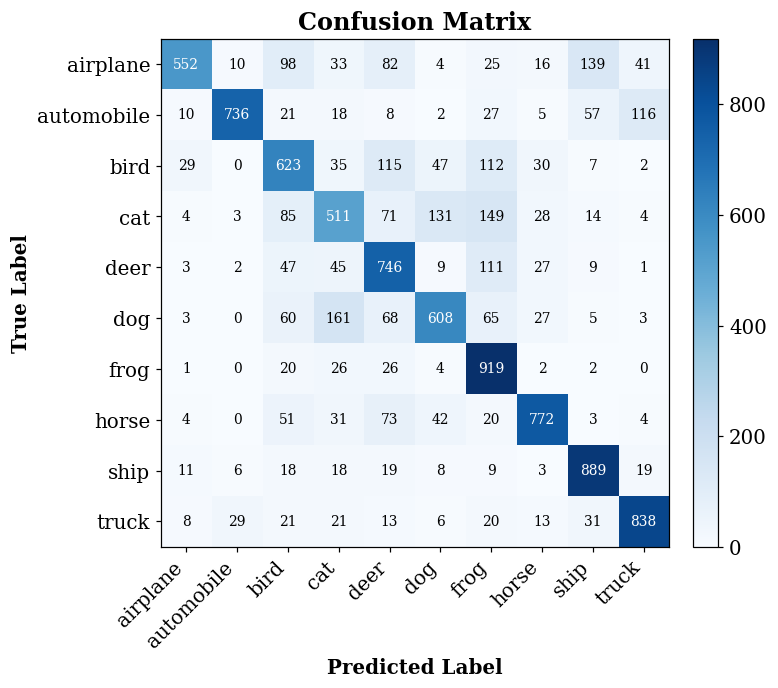
\includegraphics[width=0.7\textwidth]{figures/11_confusion_matrix.png}
\end{center}

The confusion matrix reveals which classes are most frequently confused with one another are visually similar classes such as cat/dog and deer/horse show higher off-diagonal values, while structurally distinct classes such as airplane, automobile, and ship are classified with higher accuracy.

\vspace{6mm}
\section*{8. Additional Exercises}

\textbf{1. Output Size Calculation}

Given: $64\times64$ image, $5\times5$ kernel, stride $=2$, padding $=2$.
\[
N=64,\ F=5,\ P=2,\ S=2
\]
\[
\text{Output Size}=\left\lfloor\frac{64-5+2(2)}{2}\right\rfloor+1=\left\lfloor\frac{63}{2}\right\rfloor+1=31+1=32
\]

Result: The output feature map size is $32\times32$.\\


\vspace{4mm}
\textbf{2. Trainable Parameter Calculation}

Given: 64 filters of size $3\times3$, RGB input (3 channels).
\[
(3\times3\times3+1)\times64=(27+1)\times64=1792
\]

Result: The convolution layer has 1,792 trainable parameters.\\


\vspace{4mm}
\textbf{3. ReLU vs Sigmoid Activation Comparison}

\begin{center}
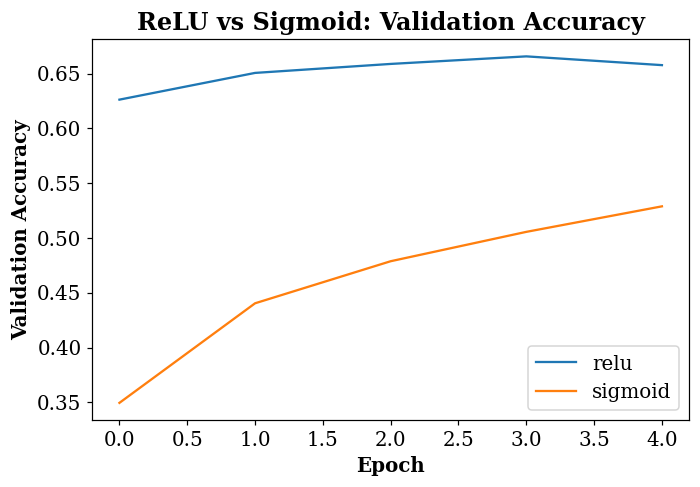
\includegraphics[width=0.8\textwidth]{figures/12_relu_vs_sigmoid.png}
\end{center}

The ReLU model learns faster and usually reaches a higher accuracy than the Sigmoid model. ReLU helps reduce vanishing gradient problem, by preserving positive gradients, while Sigmoid shrinks a few positive gradients to very small values, causing vanishing gradients problem.\


\vspace{4mm}
\textbf{4. Max Pooling vs Average Pooling: Full Training Comparison}

\begin{center}
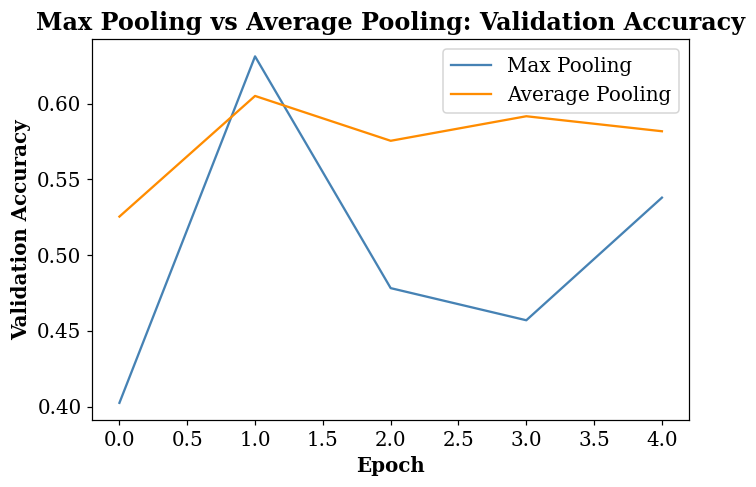
\includegraphics[width=0.8\textwidth]{figures/13_maxpool_vs_avgpool_training.png}
\end{center}

Max Pooling model performs slightly better on validation accuracy compared to Average Pooling. Max Pooling keeps the strongest activations from each region, which helps retain important features for classification. Average Pooling instead takes the average of the values, giving a smoother representation but losing some of the stronger features.\

\vspace{4mm}

\textbf{5. Effect of Increasing Filter Count (16 $\rightarrow$ 64)}

\begin{center}
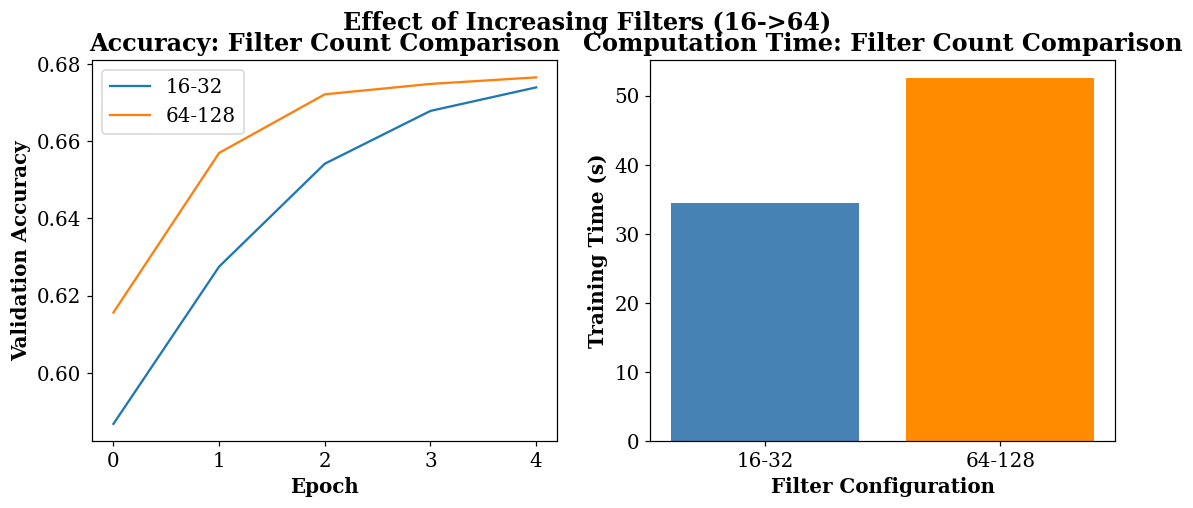
\includegraphics[width=0.8\textwidth]{figures/14_filter_count_comparison.png}
\end{center}

Increasing the filter count from 16 to 64 gives the CNN more filters to detect different features in the images. This can improve the model's accuracy, but it also increases the number of parameters and the time required for training. The results show the trade off between getting better performance and keeping the model efficient.

\vspace{6mm}
\section*{9. Discussion}

\textbf{1. Why is convolution preferred over fully connected layers for images?}

Convolution works well for images because it goes through small parts of the image at a time detects patterns such as edges and textures. Also, the number of parameters is less, as the filter keeps moving throughout the image. The same filter is used across different parts of the image, so the number of parameters is much smaller than in a fully connected layer. Fully connected layers use multiple parameters, as every layer is interconnected. It also loses spatial information about the image.

\vspace{4mm}
\textbf{2. How does stride affect the feature map size?}

Stride decides how much spaces the filter should move after each convolution. Bigger values of stride mean that the kernel moves more spaces every step, and hence produces a smaller feature map.  The output size can be calculated using $\frac{N-F+2P}{S}+1$, where S is the stride. Increasing the stride reduces the spatial size and computation, but too large a stride can cause some important image details to be lost.

\vspace{4mm}
\textbf{3. What is the role of padding?}

Padding adds extra pixels around the edges of the input image. This is done to preserve the size of the feature map, maintaining input size after convolution. Generally, it adds pixels of value 0 along the edges of the image. It also allows the pixels near the edges to be considered properly instead of being used less often than the pixels in the middle.

\vspace{4mm}
\textbf{4. Why is pooling used?}

Pooling reduces the size of a feature map while keeping the important information. This reduces the amount of computation in the later layers and can also help prevent overfitting. It also makes the network less affected by small changes in the position of a feature.

\vspace{4mm}
\textbf{5. How do feature maps represent image characteristics?}

A feature map shows where a particular filter finds a useful pattern in an image. For example, a filter in an early layer may detect edges or colour changes. As we move to deeper layers, the network combines these simple features to detect more complex patterns and objects.

\vspace{4mm}
\textbf{6. Why do CNNs require fewer parameters than MLPs?}

CNNs use the same set of kernel weights at different positions in the image instead of using separate weights for every connection. They also work with small local regions rather than connecting every pixel to every neuron. MLPs have fully connected layers, making the number of parameters very high. Because of this, CNNs can learn useful image features with far fewer parameters than a fully connected MLP.

\vspace{6mm}
\section*{10. Conclusion}

In this experiment, the main building blocks of Convolutional Neural Networks, including convolution, activation, pooling, and fully connected layers, were implemented and tested using the CIFAR 10 dataset. Effects of paramaters like stride, padding and kernel size, were also implemented and studied. The results matched the expected output size given by the formula. Visualizing the feature maps showed how different filters can detect different patterns in an image. The comparison between Max Pooling and Average Pooling also showed that Max Pooling keeps stronger features, while Average Pooling produces a smoother representation.

A CNN with the architecture Conv $\rightarrow$ ReLU $\rightarrow$ MaxPool $\rightarrow$ Conv $\rightarrow$ ReLU $\rightarrow$ MaxPool $\rightarrow$ Flatten $\rightarrow$ Dense $\rightarrow$ Softmax was trained on CIFAR 10 for 20 epochs using the Adam optimizer. The model was then evaluated using classification metrics and a confusion matrix. The additional experiments helped in understanding how the number of parameters changes, how different activation functions affect training, and how increasing the number of filters can improve accuracy while also increasing computation. Overall, the experiment gave practical experience with the basic concepts behind CNNs and showed how different design choices affect the model's performance.

\vspace{6mm}
\section*{11. References}
\begin{enumerate}
\item Goodfellow et al., \emph{Deep Learning}.
\item Bishop, \emph{Pattern Recognition and Machine Learning}.
\item Haykin, \emph{Neural Networks and Learning Machines}.
\item TensorFlow Documentation.
\item CIFAR-10 Dataset Documentation.
\end{enumerate}

\end{document}